54. \begin{figure}[ht!]
\center{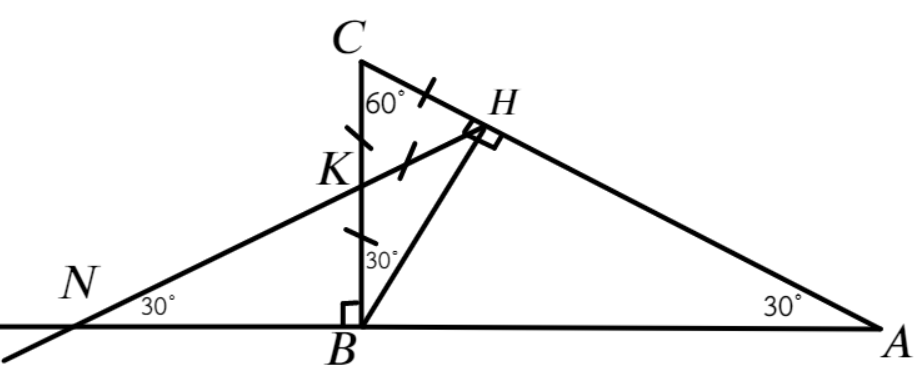
\includegraphics[scale=0.35]{g54.png}}
\end{figure}\\
Раз угол $A$ равен $30^\circ,$ угол $B$ равен $90^\circ-30^\circ=60^\circ.$ Треугольник $KCH$ является равнобедренным и один из его углов равен $60^\circ,$ значит он равносторонний и все его углы равны $60^\circ.$ Тогда $\angle NKB=\angle CKH=60^\circ$ (вертикальные), а $\angle KNB=90^\circ-60^\circ=30^\circ.$ По теореме о катете, лежащем напротив угла в $30^\circ$ для треугольников $BCH,\ KNB$ и $ABC$ имеем $CB=2CH=2KC\Rightarrow KB=CB-KC=KC,\ KN=2KB,\ AC=2CB=4KB.$ Тогда $AH=AC-CH=4KB-KB=3KB,$ а значит $AH:KN=3KB:2KB=3:2.$\\
